\documentclass[a4paper,12pt]{article}
\usepackage{a4wide}
\usepackage{ucs}
\usepackage[utf8x]{inputenc}
\usepackage{xcolor}
\usepackage[ czech,english]{babel}
\usepackage[pdftex, final]{graphicx}
% \usepackage[pdftex, final, colorlinks=true]{hyperref}
\usepackage{alltt}
\usepackage{paralist}
\usepackage{mdwlist}\usepackage{subfig}
\usepackage[final]{pdfpages}
\usepackage[final,pdftex, colorlinks=false]{hyperref}

%%%%%%%%%%%%%%%%%%%%%%%%%
% pro podmineny preklad
% false je defaultně


% \newif\ifbc % Pouze do bakalářské práce
%  \bctrue

%%%%%%%%%% fancy %%%%%%%%%%%
\usepackage{fancyhdr}

\fancyhead[L]{ČVUT v Praze}

\setlength{\headheight}{16pt}

% \usepackage{stdpage}


%%%%%%%%%%%% rozmery %%%%%%%%%%%%%%%%%%
\usepackage[%
%top=40mm,
%bottom=35mm,
%left=40mm,
%right=30mm
top=40mm,
bottom=35mm,
left=35mm,
right=25mm
]{geometry}


\renewcommand\baselinestretch{1.3}
\parskip=0.8ex plus 0.4ex minus 0.1 ex

%%%%%%%%%%%%%% Listings %%%%%%%%%%%%%%%%%
\usepackage[final]{listings}

\definecolor{lightGrey}{RGB}{250,250,250}
\definecolor{darkGrey}{RGB}{100,100,100}
\lstdefinelanguage{psmap}
{morekeywords={scale, mapinfo, maploc, where, end, font, fontsize, color,
border, raster, width, paper,
vpoints, vareas, vlines, symbol, size, rgbcolumn, sizecolumn, cwidth,
rotatecolumn, },
morekeywords=[2]{y, n, none},
morecomment=[l]{\#},
}
\lstdefinestyle{psmap}{
   language=psmap,
   basicstyle={\sffamily},
   keywordstyle=[1]{\bfseries},
   keywordstyle=[2]{\color{black}},
   commentstyle={\itshape},
   frame=lines,
   backgroundcolor=\color{lightGrey},
}
\lstdefinestyle{psmapInline}{
   language=psmap,
   basicstyle={\sffamily},
   keywordstyle=[1]{},
   keywordstyle=[2]{\bfseries\color{darkGrey}},
   commentstyle={\itshape},
   frame=lines,
   backgroundcolor=\color{lightGrey},
}


\lstdefinestyle{script}{
    language=bash,
    basicstyle={\ttfamily\footnotesize},
    keywordstyle={\bfseries},
    commentstyle={\itshape},
    frame=lines,
    backgroundcolor=\color{lightGrey}
}
\lstnewenvironment{psmap}[1][]
{\lstset{style=psmap,
   #1}}
   {}
\renewcommand{\lstlistingname}{Ukázka}
%%%%%%%%%%%%%%%%%%%%%%%%%%%%%%%%%

\newcommand{\klicslova}[2]{\noindent\textbf{#1: }#2}
\newcommand{\modul}[1]{\emph{#1}}
%\newcommand{\instr}[1]{\lstinline[style=psmapInline]|#1|}
\author{Matěj Krejčí}
% \pagecolor{darkGrey}
\newcommand{\necislovana}[1]{%
\phantomsection
\addcontentsline{toc}{section}{#1}
\section*{#1}
\markboth{\uppercase{#1}}{}
}
\hyphenation{ArcGIS}

%%%%%%%%%%%%%%%%%%%%%%%%%%%%%%
\begin{document}
\pagestyle{empty}


\begin{center}
%napisy
\newcommand{\napisCVUT}{České vysoké učení technické v Praze}
\newcommand{\napisFS}{Fakulta stavební}
\newcommand{\napisObor}{Obor geoinformatika}
\newcommand{\napisKatedra}{Katedra geomatiky}
\newcommand{\napisVedouci}{Ing. Martin Landa Ph.D.}
\newcommand{\napisAutor}{Matěj Krejčí}
\newcommand{\napisDatum}{Praha 2014}
\newcommand{\napisNazevI}{Analýza a vizualizace srážkových dat }
\newcommand{\napisNazevII}{z mikrovlnných telekomunikačních spojů pomocí GIS}
\newcommand{\napisNazevAjI}{Analysis and vizualization of rainfall data from}
\newcommand{\napisNazevAjII}{microwave links using GIS}
\newcommand{\napisBakalarka}{Bakalářská práce}
\newcommand{\napisPraha}{Praha 2014}
%
% prikazy
%\newcommand{\velka}[1]{\uppercase{#1}}
\newcommand{\velka}[1]{\textsc{#1}}
%
% 
\newif\ifpatitul
\patitultrue

\ifpatitul
{\Large\velka{\napisCVUT}}\\
\velka{\Large\napisFS}\\
\vfill
{\LARGE\velka{\napisBakalarka}}
\vfill
{\large\napisPraha\hfill\napisAutor}
\newpage
\fi%patitul


{\Large\velka{\napisCVUT}}\\
{\Large\velka{\napisFS}}\\
{\Large\velka{\napisObor}}
\vfill

\includegraphics[width=3cm]{logo_cvut_cb} %~
\vfill
{\Large\velka{\napisBakalarka}}\\
{\Large\velka{\napisNazevI\\
\napisNazevII}}\\
{\large\velka{\napisNazevAjI\\
\napisNazevAjII}}
\vfill
{\large%
Vedoucí práce: \napisVedouci\\
\napisKatedra\\
\bigskip
\napisDatum\hfill\napisAutor}
\end{center}

\newpage
\definecolor{navodotisk}{RGB}{10,10,10}
\newcommand{\vlozZadani}{%
\Huge\textcolor{navodotisk}{\textsf{\textbf{ZDE VLOŽIT ORIGINÁLNÍ ZADÁNÍ}}}%
}
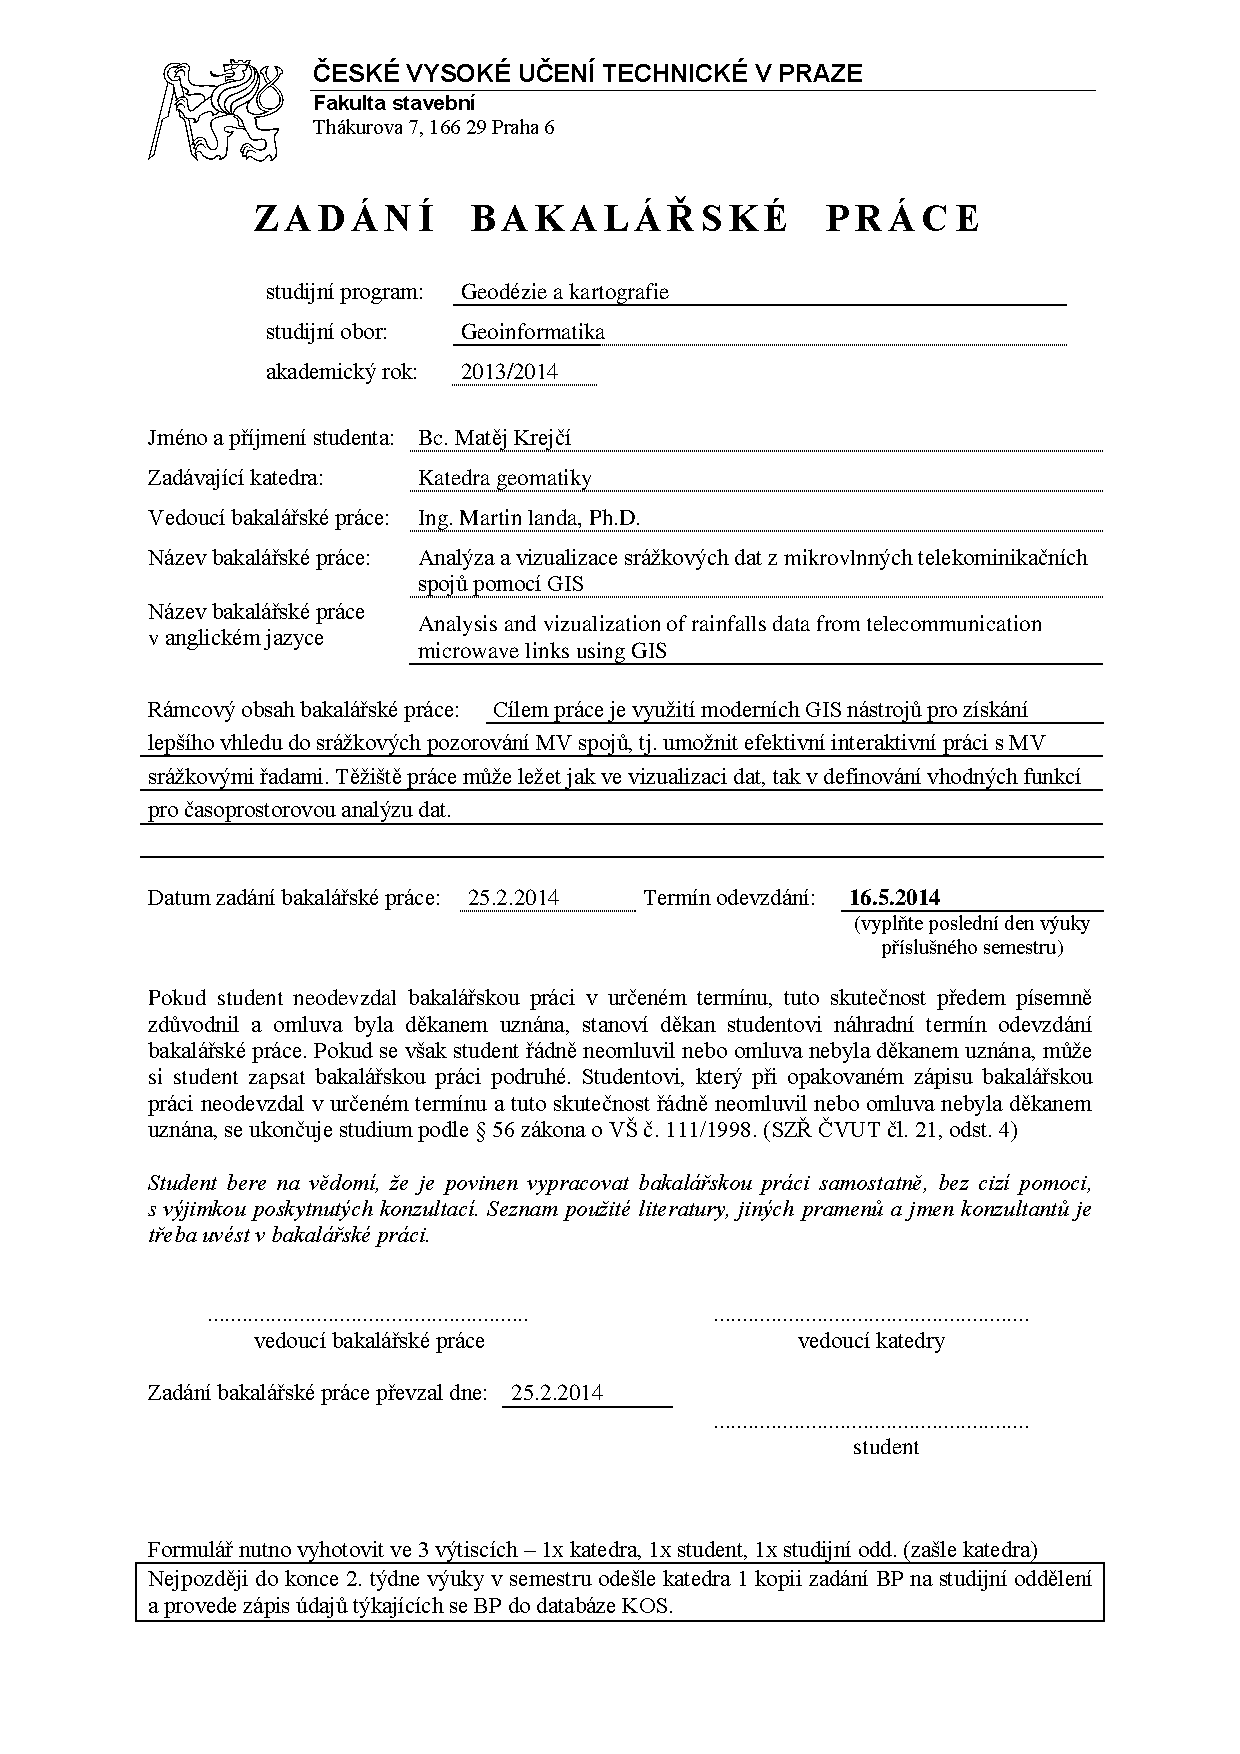
\includepdf[picturecommand={\put(100,200){\vlozZadani}}]{../formulare/zadanibp}
 % resi si zalomeni sam


\begin{abstract}
Cílem této bakalářské práce je modelování dešťových srážek z dat mikrovl\-
nných spojů telekomunikačních operátorů. Data ke zpracování jsou uloženy pomocí relační databáze PostgreSQL.
K modelování srážek byl použit systém GRASS GIS Python API. Modul implementuje rekonstrukce dešťových srážek na základě uživatelské konfigurace. Další funkcionalitou je dávkové zpracování grafického výstupu srážek. Hlavní přínos modulu je v předzpracová\-ní dat pro hydrologické a meterologické analýzy s využitím nástrojů GIS.
\bigskip

\klicslova{Klíčová slova}{GIS, GRASS GIS, Python, PostgreSQL, dešťové srážky, časoprostorová analýza, interpolace}

\end{abstract}

\selectlanguage{english}
\begin{abstract}
TODO 
\bigskip

\klicslova{Keywords}{GIS, GRASS GIS, Python, PostgreSQL, precipitation, temporal analysis,interpolation}

\end{abstract}
\selectlanguage{czech}


\newpage
\newcommand{\odsaditodzhora}{\hskip1pt\vfill}

\odsaditodzhora
\noindent Prohlášení
%%% MK: predelano po revizi
Prohlašuji, že bakalářskou práci na téma „Analýza a vizualizace srážkových dat z mikrovlnných telekomunikačních spojů pomocí GIS“ jsem vypracoval samostatně. Veškerá použitá literatura je uvedena v seznamu zdrojů.

\begin{flushleft}
\begin{tabular}{cp{0.3\textwidth}c}
V Praze dne .................
& 
&
..................................
\\
&&
(podpis autora)
\end{tabular}

\end{flushleft}
\newpage

\odsaditodzhora
\noindent Poděkování

Tady bude podekovani

\newpage

\newpage
\tableofcontents


\newpage
\pagestyle{fancy}

\necislovana{Úvod}

Enviromentální modelování se v posledních době rozšířilo ve velkém měřítku. Velkou částí k tomu přispěla dostupnost informačních technologií a s ním spojený zájem vědeckých pracovišť o tento obor. Již ze samotného názvu vyplývá, že enviromentální modelování se zabývá životním prostředím a jeho modelováním. Pod tento obor spadá nespočetné množství podoborů, které se především liší kladením rozdílných otázek. Specifikovat jednotnou definici pro enviromentálního modelování je pro jeho multidisciplinaritu velmi obtížné. Modelování přírodních procesů vzniklo v důsledku zájmu člověka o pochopení přírody. Studium a simulace přírodních jevů z oborů fyzikálních, matematických, biologických a chemických v dnešní době velmi usnadňuje člověku život a v některých regionech je člověk i přímo závislý na zprostředkovaných výsledcích, které jsou produktem enviromentálních modelů. 

Modelování dešťových srážek(dále srážek) je jednou z velkých disciplín z oboru enviromentálního modelování. Když se poohlédneme do první poloviny 19. století, tak právě meteorologie byla jednou z prvních disciplín, která definovala pojem enviromentální modelování, tak jak ho chápeme nyní. Modelování srážek na zemském povrchu se s vývojem klimatu stává v poslední době důležitým úkolem. Oproti rozvoji fyzikálně numerických modelů a to především díky stále se zvyšujícím výpočetním výkonům počítače, nebyl technologické pokrok ve sběru srážkových dat v posledních desetiletích takřka zaznamenán. Pracovníky meteorologických a hydrologických ústavů ve vývoji brzdí nedostatečná, nepřesná a neaktuální srážková data, které jsou jedním z hlavních vstupu pro další modely. Studie z posledních let poukazují na možnost využití mikrovlnných(dále MV) spojů vysílačů telekomunikačních operátorů ke sběru srážkových dat. Tento zdroj je levnější a přesnější než sběr pomocí radaru.\cite{radar_meterology} Největší potenciál sběru srážkových dat v reálném čase je ve vylepšení městských odtokových modelů. Pro efektivitu těchto modelů je sběr dat v reálném čase nutností.

Hlavním cílem této práce je vyvinutí nástroje pro zpracování hrubých dat z MV vysílačů v prostředí GIS, čímž se zpřístupní nespočet dalších analýz pro vývoj tohoto poměrně mladého výzkumu. Téma práce bylo založeno na požadavcích zpracovatele projektu, který se zabývá problematikou odhadu srážek z MV zdrojů v rámci projektu TeleMAS v souvislosti s modelováním srážko-odtokových procesů v městských povodích. Tento projekt je řešen v úzké vědecké spolupráci s ETH-Eawag a odborné spolupráci se společnostmi T-Mobile a Veolia ČR a nyní nově s Ericsson Research (Sweden).  

 




\newpage
\section{Měření dešťových srážek}
První část této kapitola má za cíl přiblížit čtenáři současné metody měření dešťových srážek. Liší se především v přesnostech, časové ?variabilitě? a vhodností výstupu pro další využití. Tento úvod do problematiky měření srážek by měl napomoct k lepšímu pochopení výhod či nevýhod metody odhadu srážek pomocí MV, která bude v druhé části kapitoly představena a s těmito metodami porovnána. Nejdříve se ale podíváme trochu do historie.
\subsection{Historie stručně}
Podíváme-li se do historie a opomeneme nejasné zmínky měření srážek z období 100 n.l. v Palestině, dostaneme se k přelomu 14-15. století na území Korei za vlády krále Sejong.\cite{sejong} První náznak vynalezení srážkoměru vzniklo z rozhodnutí, že místo výkopů v pudě pro kontrolu vlhkosti, bude efektivnější mít standardizovaný nástroj na měření deště. Oproti neznámým metodám měření se alespoň dochovaly zmínky o rozměrech a tvaru srážkoměru. Hlavním účelem měření bylo efektnější rozhodování panovníka při určování výše daní z obdělávaných polí farmářů. S dalším mezníkem v historii vývoje srážkoměrů měl co do činění angličan Sir Christopher Wren v letech 1661.\cite{wren} Vynalezl srážkoměr, který fungoval na principu vážení kapaliny, čímž se velmi podobal současným standardům(jeden gram vody je ekvivalentem ke krychlovému centimetru objemu vody). První měření srážek v metrických jednotkách učinil pan Benjamin Franklin. Bylo tomu v letech 1790, kdy byl poprvé metrický systém definován a stejný rok se stal i panu Frenklin osudný. Od té doby se principiálně srážkoměry nemění. Samozřejmostí je, že se v průběhu staletí dochází k jejich  zpřesňování přesnosti měření, standardizaci a v posledních desetiletích především k automatizaci.

Mezníkem ve sběru srážkových dat se bezesporu stal radar. Jak již bylo zmíněné, že nic nevzniká bez vyšší motivace, v tomto případě to byl vojenský konflikt. Při druhé světové válce byl do provozu uveden první experimentální radar, který sloužil k metrologickému pozorování. Přesněji tomu bylo roku 1930 v USA. \cite{flash_floods} Roku 1959 následovalo první vytvoření radarové sítě WRS-57 v USA. Postupem času se poté rozšíří metoda odhadu srážek radarem zcela globálně. 

Nástup satelitních družic se datuje v šedesátých letech 19. století. Logickou návazností na první satelitní družice vzniká obor, který dnes známe pod pojmem dálkový průzkum země(DPZ). Jedná se o zcela nový obor 20. století vyplývající z technologického pokroku. Oproti výše zmíněným metodám není DPZ striktně zaměřen pouze pro hydrometeorologické účely. Jednotlivé družice jsou svým vybavením určeny pro měření různých veličin a jevů. V této kapitole se dále budeme soustředit především na družice metrologické. Je zde důležité zmínit historicky první meteo družici Vanguard 2 z let 17. února 1959\cite{vanguard} a o mnoho úspěšnější družici 1. dubna 1960 s označením TIROS-1.
     



\subsection{Současné nástroje na měření a odhad srážek}

\paragraph*{Dešťové srážky}jsou definovány jako kondenzace vodní páry v kapalném nebo pevném stavu, které padají z oblohy či kondenzují přímo na zemském povrchu. Srážky mohou mít formu sněhových vloček- pevné skupenství, nebo formu dešťových kapek- kapalné skupenství. Množství srážek bývá udáváno v milimetrech kapalné vody spadlé na zemský povrch.\cite{wmo}

\subsubsection{Srážkoměry}
Srážkoměr je přístroj používaný v meteorologii a hydrologii k měření srážkových úhrnů. Funkčností se srážkoměry dělí na dešťové  a na srážkoměry, které měří i srážky pevného skupenství. Tyto srážky se přeměňují na ekvivalent vody a až pote se měří. Je zde důležité podotknout, že produktem srážkoměrů jsou bodové srážkoměrné data.


\begin{description} 
\item[Ombrometr]je jeden z nejednodušších typů srážkoměru. Je tvořen válcem s nálevkou, která převádí padající srážky do nádoby uvnitř válce. Srážkový úhrn se změří přelitím obsahu nádoby do kalibrovaného odměrného válce. Pro zachycení sněhu se z ombrometu sundá nálevka a sníh se nechává roztát. Tyto srážkoměry se využívají velmi zřídka.

\textbf{Výhody} jsou zde pouze v jednoduchosti obsluhy bez nutnosti kalibrace a také i nejmenší náklady na pořízení.
   
\textbf{Nevýhody} jsou především nutnosti asistovaného měření. Dále pak také v nefunkčnosti přes zimní období, kdy srážkoměry zamrzají. 
\end{description}

\begin{description} 
\item[Ombrograf]se skládá z nádoby s plovákem a registračního zařízení. Srážky stékají do nádoby s plovákem, na který je napojeno registrační zařízení, které zapisuje údaj na otáčející se roli papíru. Takto vytvořený záznam se nazývá ombrogram. Záznam popisuje průběh celkového množství srážek v čase, z něho se dá odvodit intenzita srážky. Podle doby otočky bubnu kolem své osy rozlišujeme přístroje s týdenním (buben s registrační páskou se otočí o jednu otočku asi za 168 hodin) a jednodenním (otočka asi 24 hodin) chodem.\cite{chmu_navod}

\textbf{Výhody} ombrografu jsou v možnosti kontinuálního sledování srážkových úhrnů.

\textbf{Nevýhody} těchto měřících stanic jsou v přesnosti. Údaje z nich získané jsou většinou méně přesné než ze základních přístrojů. Dalším faktorem je nutnost pravidelné obsluhy, která a spočívá v natažení hodinového stroje, výměny pásky a doplnění registračního inkoustu.
\end{description}

\begin{description} 
\item[Člunkový srážkoměr] je jeden s nejvíce používaných srážkoměrů současné doby. Princip jeho funkčnosti je založen na překlápěcím člunku, jehož jedna polovina se po dosažení úhrnu srážek 0.1 mm překlopí, čímž se polovina vyprázdní a začne se naplňovat druhá polovina. Takto se cyklus opakuje. Stanice překlopení zaznamenává a z počtu pulsů za určitý čas se vypočítají srážkové úhrny. Některé typy těchto srážkoměrů jsou vybaveny vyhříváním a tudíž mohou měřit i tuhé srážky.

\textbf{Výhody} těchto srážkoměrů jsou bezesporu v automatizovaném běhu stanice, bez nutných krátkodobých obsluh. 

\textbf{Nevýhody} člunkových srážkoměrů jsou při prudkých deštích, kdy mohou s nedostatečně rychlého překlápění člunku výsledné úhrny srážek být podhodnoceny.\cite{sevruk}
\end{description}

\begin{description} 
\item[Váhový srážkoměr] funguje na principu vážení kapaliny. Váhový srážkoměr se skládá z nádoby, která je postavena na váze. Srážkoměr do nádoby zachycuje kapalinu, která je vážena tenzometrickou váhou napojenou na řídící elektronickou jednotku.

\textbf{Výhody} jsou v přesnosti měření a konstrukci srážkoměru. Tuhé srážky váhový srážkoměr zachytí a vyhodnotí bez prodlevy nutné pro jejich roztátí. Rovněž přesnost váhového srážkoměru není závislá na intenzitě srážek oproti srážkoměru s překlápěcím člunkem, kde přesnost se vzrůstající intenzitou klesá.

\textbf{Nevýhody} těchto zařízení jsou ve vyšší pořizovací ceny a díky složitostí mechanizmu také vyššími náklady na údržbu.
\end{description}


\subsubsection*{Chyby při měření srážkoměrem} 
Měření srážek srážkoměry jsou ovlivněny mnoha faktory, které určují konečnou přesnost a spolehlivost tohoto typu měření.
\begin{description} 
\item[Přístrojové chyby] se přesněji odvíjejí od jednotlivých zařízení. Přesnost u Ombrografů se pohybuje okolo 0.2 mm do  úhrnu srážek 20 mm za hodinu. Člunkové srážkoměry mají chybu měření 0.5 mm pro úhrn 20mm  srážek za hodinu. Chyby se zvyšují s výšší intenzitou srážek. Při srážkách 150 mm za  hodinu je chyba větší než 3\%. \cite{wmo}
\item[Proudění vzduchu] je jedním z nejvíce nežádoucích vlivů, které nejvýznamněji ovlivňují přesnost měření. Zamezení tomuto vlivu je velice obtížné zabránit. V nejlepším případech by mělo být ve vodorovné poloze. Z toho plynou nároky na umístění přístroje. Minimalizovat nežádoucí proudění větru se řeší pomocí několika pravidel: umístění mimo strmá území a zastavěné lokality. Umístění zařízení co nejníže k zemi. Umístění na trávník k zabránění vstupu odrážejících se kapek. 
\item[Chyby ze smáčení] jsou způsobeny nedostatečné hydrofobním povrchem nádob a v případě srážkoměru s člunky v neúplném vylití kapaliny při vyprazdňování. Dalším faktorem jsou přírodní vlivy, především zachycování nečistot, prachu, pavučin a dalších materiálů absorbující kapalinu. Z toho se tvoří zbytkové vody, které tvoří další chyby. 
\item[Chyby z odpařování] mají vyhřívané člunkové srážkoměry. Jsou způsobeny vypařováním vody s člunku což při malých srážkových úhrnech způsobuje značné chyby.
\item[Sklápění člunku] je hlavním problémem člunkových srážkoměru. Při velkých deštích vstupuje do voda do trychtýře i když je člunek ve stavu vylévání. To způsobuje odvádění vody která nebyla změřena. 

\end{description}

\subsubsection{Meteorologický radar}
\paragraph*{Princip}
radaru je založen na dopplerovském jevu.\cite{radar_meterology} Vysílací zařízení generuje opakovaně v řádu mikrosekund krátké elektromagnetické pulsy, které jsou vysílány ve tvaru úzkého svazku do atmosféry. Elektromagnetická energie se v atmosféře odráží jak od meteorologických objektů tak i objektů jiných(letadla, terén). Část elektromagnetické energie, která není pohlcena nebo odražena jiným směrem je detekována přijímačem radaru. Ze známé polohy antény, síly signálu a doby mezi jeho vysláním a přijetím se určí vzdálenost a poloha objektu, srážky. 
Pro meteorologické účely se využívá především dlouhých vlnových délek v rozsahu 1-10 cm, kterému odpovídá přibližně desetinásobek velikosti průměrných dešťových kapek nebo pevných částic. Kratších vlnových délek se využívá k zaznamenání menších částic jako je například mlha. Zde nastává problem v rychlém oslabení signálu.\cite{doppler}

\paragraph*{Srážková data}se měří obvykle v intervalu 5-15 minut. Horizontální rozlišení dat bývá 2×2 km, vertikální 1 km. Toto prostorové rozlišení je nutné, aby bylo možné zachytit jednotlivá srážková jádra přeháněk. Radarové odrazy jsou interpretovány plošně a jsou zobrazovány v barevné stupnici intenzit srážek.
\paragraph*{Rozsah} meteorologického radaru bývá okolo 250 km. Hodnoty naměřené radarem mohou být použity pro odhad okamžitých intenzit srážek do vzdálenosti přibližně 150 km od radaru.\cite{kohout}






\subsubsection{Satelitní družice}
\subsection{Mikrovlnné spoje}
\subsubsection{Problematika}
\subsubsection{Výpočet srážky}
\subsection{Srovnání metod měření srážek}
\subsubsection{Chyby}
\subsubsection{Konzistence dat}

\subsubsection{Potenciál v hydrometeorologii}
\section{Interpolace srážek}
\section{GRASS GIS modul}
\subsection{Funkcionalita}
\subsection{Implementační nástroje}
\subsubsection{GRASS API}
\subsubsection{PostgreSQL}
\subsubsection{Psycopg?}
\subsection{Vstup}   
\subsection{Výstup}
\section{Časoprostorové analýzy}
\subsection{Využitelnost}
\section{Závěr}
\section{Příloha}
\subsection{Dokumentace}
\subsection{Uživatelská příručka}




%\begin{enumerate*}
   % \item nastavit region na zvolenou rastrovou či vektorovou mapu
    %\item nastavit uložený region (\emph{named region})
   % \item nastavit aktuální výpočetní region
  %  \item zvolit souřadnice středu mapy a měřítko (nastavení regionu
 %   se automaticky vypočítá)
%\end{enumerate*}





\necislovana{Závěr}

Cílem této práce bylo 


\newpage
\necislovana{Seznam použitých zkratek}

\begin{tabular}{ll}
\textbf{GIS}& Geographic Information System (Geografický informační systém)\\
\textbf{GRASS}& Geographical Resources Analysis Support System\\
\textbf{GUI}& Graphical User Interface (Grafické uživatelské rozhraní)\\
\textbf{XML}& Extensible Markup Language\\



\end{tabular}


\newpage
\renewcommand\baselinestretch{1.2}
\selectfont
\renewcommand{\refname}{Použité zdroje}
\phantomsection
\addcontentsline{toc}{section}{\refname}

\begin{thebibliography}{99}
\label{literatura}




\bibitem{radar_meterology}
RAGHAVAN, S. \textit {Radar meteorology}.
31 Oct 2003. Boston: Kluwer Academic Publishers, 2003, 549 s. ISBN 14-020-1604-2. 

\bibitem{flash_floods}
SENE, Kevin. \textit {Flash floods forecasting and warning}.
2013. Dordrecht: Springer, 2013. ISBN 978-940-0751-644. 

\bibitem{vanguard}
GREEN, McLaughlin a Milton LOMASK. \textit {Vanguard - A history: succes - AND AFTER http://history.nasa.gov/SP-4202/toc2.html}.
[online]. [cit. 2014-04-03]. URL:\textless\url {http://history.nasa.gov/SP-4202/chap12.html}

\bibitem{sejong}
STRANGEWAYS, Ian.  \textit {Precipitation: theory, measurement and distribution}.
New York: Cambridge University Press, 2007, x, 290 p. ISBN 978-052-1851-176. 

\bibitem{wmo}
World Meteorological Organization. \textit{Guide to meteorological instruments and methods of observation CHAPTER 6}. WMO-No. 8. Geneva, Switzerland: World Meteorological Organization, 2008. ISBN 978-926-3100-085. 

\bibitem{wren}
ASIT K. BISWAS {Notes and Records of the Royal Society of London: The Automatic Rain-Gauge of Sir Christopher Wren} UK: The Royal Society, 1967. ISSN 00359149. 

\bibitem{sevruk}
SEVRUK, B.\textit{Niederschlag als Wasserkreislauf-element. Theorie und Praxis der Niederschlagsmessung.} 
Zurich-Nitra: Eigenverlag ETH Zurich,  2004, 200 s, ISBN 80–969343–7–6.

\bibitem{chmu_navod}
Česká republika, \textit{Návod pro pozorovatele meteorologických stanic.}
In: Metodický předpis č. 13. Ostrava, 2013. URL:\textless\url {http://old.chmi.cz/OS/pdf/metodicky_navod/MP.pdf}


\bibitem{doppler}
DOVIAK, R. J.; D. S. Zrnic , \textit{Doppler Radar and Weather Observations (2nd ed.)}
(1993), San Diego CA: Academic Press, ISBN 0-12-221420-X.

\bibitem{kohout}
KOHOUT, Jan. \textit{Zpracování a prezentace srážkových dat měřících stanic meteorologického radaru pro ČHMÚ. Informační technologie pro praxi.}
Ostrava: TANGER, 2003. s. 101-103. ISBN 80-85988-90-9.








\end{thebibliography}
\end{document}



